\section{Signal Model}
\label{sec:signal}

\begin{figure}[!b]
\centering
    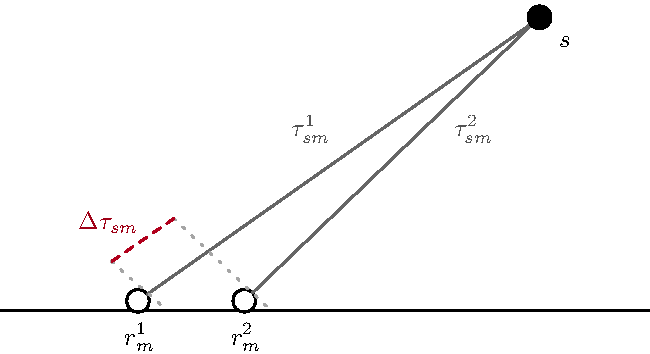
\includegraphics[scale=0.8]{data/figures/signal2}
    \caption{Direct Propagation Paths for Source $s$ and Microphone Pair $m$.}
    \label{fig:signal}
\end{figure}

The basic configuration, as depicted in Figure \ref{fig:signal}, consists of two microphones that constitute one microphone pair. The received signal $x^i_m$ at microphone $i$ of pair $m$ can be described as a linear combination of the acoustic transfer function $a^i_{sm}$, multiplied bin-wise with the source signal $v_s$, and additive white Gaussian noise $n^i_m$ in the \acrfull{stft} domain
\begin{equation}
	x_m^i(t,k)=\sum_{s=1}^{S}a_{sm}^i(t,k)\cdot v_s(t,k)+n_m^i(t,k),
	\label{eq:x}
\end{equation}

where $t\in\{1,\dots,T\}$ denotes the time-index or time-bin, $k\in\{1,\dots,K\}$ denotes the frequency-index or frequency-bin, $(m,i)$ describe microphone $i\in\{1,2\}$ of microphone pair $m\in\{1,\dots,M\}$ and $s\in\{1,\dots,S\}$ denotes the source index. For the experimental part in \autoref{chap:experiments}, the \gls{rir} is used as the time-domain equivalent to the acoustic transfer function. The direct path of the transfer function, that part corresponding to the line-of-sight, can be described as
\begin{equation}
	a_{sm}^i(t,k)\approx\frac{1}{\|\bm p_s-\bm p_m^i\|}\cdot\exp{\left(-\iota\frac{2\pi k}{K}\frac{\tau^i_{sm}}{T_s}\right)},
	\label{eq:acoustic_transfer_function}
\end{equation}

where $T_s$ is the sampling period of source signal $v_s$, $\ps$ is the position of source $s$, $\bm p^i_m$ is the position of microphone $(m,i)$, $\|\bm p_s-\bm p_m^i\|$ is the Euclidean distance between the source and the microphone position and $j$ is the imaginary unit. The signal travel time $\tau^i_{sm}$ between source position $\bm p_s$ and microphone position $\bm p^i_m$ is determined by the sound velocity $c$
\begin{equation}
	\tau^i_{sm}=\frac{\left(\|\bm p_s-\bm p_m^i\|\right)}{c},
\end{equation}

which is determined by both the type and properties of the medium the signal as travelling in as well as the temperature. To estimate the location of a source, we solve for the \gls{tdoa} $\Delta\tau_{sm}$, which we define as
\begin{equation}
    \Delta\tau_{sm}=\tau^2_{sm}-\tau^1_{sm}=\frac{\|\bm p_s-\bm p_m^2\|-\|\bm p_s-\bm p_m^1\|}{c},
\end{equation}

assuming planar wave fronts impinging on the microphones according to the far-field approximation of sound signals. From the \gls{tdoa}, the \gls{doa} can then be inferred with
\begin{equation}
    \text{DOA}=\arccos\left (\frac{c\cdot \Delta\tau_{sm}}{d_m}\right ),
\end{equation}

where arccos is the inverse of the cosine-function and $d_m$ is the Euclidean distance of the position of the two microphones $\bm p_m^1$ and $\bm p_m^2$ of microphone pair $m$
\begin{equation}
    d_m=\| \bm p_m^1-\bm p_m^2\|.
\end{equation}

The direct path of the transfer function multiplied with the source signal contains the original phase information that is needed to estimate the position of the source. The remaining part of the received signal (the reverberant tail of the transfer function multiplied with the source signal) distorts this information and will decrease the location estimation performance. 

%TODO: Klären, wann index s notwendig und wann nicht
Following \cite{Schwartz2014}, the \gls{prp} $\phi_{m}(t,k)$ of the two signals $x_{m}^1$ and $x_{m}^2$ received at each microphone pair $m$ will be used as the feature to be used for the purpose of localisation
\begin{equation}
    \phi_{m}(t,k)=\frac{x^2_{m}(t,k)}{x^1_{m}(t,k)}\cdot \left |\frac{x^1_{m}(t,k)}{x^2_{m}(t,k)}\right |.
\label{eq:prp}
\end{equation}

To understand the link of \gls{prp} and \gls{doa}, let's solve the equation for two received signals in a noiseless environment (i.e., $n^i_{m}(t,k)=0$) by inserting the definition of the received signal \eqref{eq:x} into \eqref{eq:prp} and reducing the resulting equation
%\begin{equation}
%    \frac{x^2_{sm}}{x^1_{sm}}=\frac{v_{sm}\cdot a^2_{sm}}{v_{sm}\cdot a^1_{sm}}=\frac{\|\bm p_s-\bm p_m^1\|\cdot\exp{\left(-j\frac{2\pi k}{K}\frac{\tau^2_{sm}}{T_s}\right)}}{\|\bm p_s-\bm p_m^2\|\cdot\exp{\left(-j\frac{2\pi k}{K}\frac{\tau^1_{sm}}{T_s}\right)}}=\exp{\left ( j\frac{2\pi k}{K}\frac{(\tau^1-\tau^2)}{T_s}\right )}
%\end{equation}

\begin{equation}
    \phi_{m}(t,k)=\exp{\left ( -j\frac{2\pi k}{K}\frac{\tau_{m}^1-\tau_{m}^2}{T_s}\right )}.
\end{equation}

The amplitude has been eliminated by multiplication with $|x^1(t,k)|\ /\ |x^2(t,k)|$. The \gls{prp} feature can therefore be interpreted as the effect the difference in signal travel time of different source signals has on the phase difference that can be calculated at each microphone pair.

\paragraph{W-disjoint Orthogonality}
The sources are assumed to exhibit W-disjoint orthogonality in the \gls{stft} domain \cite[p.~393]{Schwartz2014}, \cite{Rickard2006}. This means that the source signals do not overlap in the \gls{stft} domain. For two sources $s\in\{1,2\}$ and their respective source signals $v_s(t,k)$, this assumption can be formalised as
\begin{equation}
    v_1(t,k)\cdot v_2(t,k)=0~\forall~t,k.
\end{equation}

In reality, this assumption does not fully hold true but is approximated by speech signals, as these are considered to be sparse in the time-frequency domain, meaning most parts of the signal are equal to zero. For the mixture of multiple source signals it is then further assumed, that each time-frequency bin is dominated by only one source, which allows for spatial seperation of the received signal's components and subsequent source localisation. We will see that with increased reverberation and number of sources simultaneously simulated, this assumption is challenged, as the received signal will be less and less sparse.